\documentclass[a4paper, 12pt]{report}
\renewcommand{\baselinestretch}{1.5}
\usepackage[utf8]{inputenc} % Change according your file encoding
\usepackage[margin=1in]{geometry}
\usepackage[pdftex]{graphicx}
\usepackage{geometry}

\usepackage{latexsym}

\usepackage{etoc}
\usepackage{blindtext}
\usepackage{url}
\usepackage{listings}
\usepackage{anyfontsize}
\usepackage{titlesec,smartdiagram}
\usepackage{lastpage}
\usepackage{fancyhdr}
\usepackage{tocloft}
\usepackage{comment}
   
\usepackage{geometry}
\geometry{
left=2.2cm,
 top=2.54cm,
 bottom=2.921cm,
 right=1.5cm
 }

%code is missing

%opening

\begin{document}
\begin{titlepage}
\centering
	{\bfseries\fontsize{16pt}{16pt}\selectfont COLLEGE ACADEMIC MANAGEMENT SYSTEM\par}
\vspace{.5cm}
	{\fontsize{12pt}{12pt}\selectfont\bfseries PROJECT REPORT Submitted by \par}
	\vspace{.3cm}
	\begin{center}
	{\fontsize{14pt}{14pt}\selectfont\bfseries ARYASREE S \par}
	\vspace{.2cm}
	{\fontsize{12pt}{12pt}\selectfont\bfseries (RegNo:KVE17MCA008 )\par}
        {\fontsize{14pt}{14pt}\selectfont\bfseries  RENJITHA R \par}
\vspace{.2cm}
{\fontsize{12pt}{12pt}\selectfont\bfseries (RegNo:KVE17MCA018)\par}
\vspace{.2cm} 
{\fontsize{14pt}{14pt}\selectfont\bfseries SARITHA M DHARAN\par}
\vspace{.2cm}
{\fontsize{12pt}{12pt}\selectfont\bfseries (RegNo:KVE17MCA020)\par}
	\vspace{.5cm}
\end{center}
{\fontsize{12pt}{12pt}\selectfont\bfseries to \par}
	{\fontsize{12pt}{12pt}\selectfont\bfseries the APJ Abdul Kalam Technological University\par}
{\fontsize{12pt}{12pt}\selectfont\bfseries in the partial fulfilment of the requirements for the award of the Degree \par}
{\fontsize{12pt}{12pt}\selectfont\bfseries of  \par}
{\fontsize{12pt}{12pt}\selectfont\begin{textit} Master of Computer Applications\end{textit} \par}
\includegraphics[width=150pt]{Sng}\par\vspace{0.2cm}
% Bottom of the page
{\fontsize{14pt}{14pt}\selectfont DEPARTMENT OF COMPUTER APPLICATIONS \par}
    \vspace{0.2cm}
	{\fontsize {14pt}{14pt}\selectfont\bfseries Sree Narayana Gurukulam College of Engineering \par}
	\vspace{0.2cm}
	{\fontsize{14pt}{14pt}\selectfont Kadayiruppu, Kolenchery \par}
{\fontsize{14pt}{14pt}\selectfont November 2019 \par}

% Bottom of the page
\end{titlepage}
%\end{document}
%\begin{document}

\begin{titlepage}
           \centering
{\bfseries\fontsize{16pt}{16pt}\selectfont COLLEGE ACADEMIC MANAGEMENT SYSTEM\par}
\vspace{.5cm}
	{\fontsize{12pt}{12pt}\selectfont\bfseries PROJECT REPORT Submitted by \par}
	\vspace{.5cm}
 		
%{\fontsize{14pt}{14pt}\selectfont BY \par}
	%\vspace{.5cm}
	\begin{center}
	{\fontsize{14pt}{14pt}\selectfont\bfseries ARYASREE S \par}
	\vspace{.2cm}
	{\fontsize{12pt}{12pt}\selectfont\bfseries (RegNo:KVE17MCA008 )\par}
        {\fontsize{14pt}{14pt}\selectfont\bfseries  RENJITHA R \par}
\vspace{.2cm}
{\fontsize{12pt}{12pt}\selectfont\bfseries (RegNo:KVE17MCA018)\par}
\vspace{.2cm} 
{\fontsize{14pt}{14pt}\selectfont\bfseries SARITHA M DHARAN\par}
\vspace{.2cm}
{\fontsize{12pt}{12pt}\selectfont\bfseries (RegNo:KVE17MCA020)\par}
	\vspace{.5cm}
\end{center}
	
{\fontsize{12pt}{12pt}\selectfont\bfseries to \par}
	{\fontsize{12pt}{12pt}\selectfont\bfseries the APJ Abdul Kalam Technological University\par}
{\fontsize{12pt}{12pt}\selectfont\bfseries in the partial fulfilment of the requirements for the award of the Degree \par}
{\fontsize{12pt}{12pt}\selectfont\bfseries of  \par}
{\fontsize{12pt}{12pt}\selectfont\begin{textit} Master of Computer Applications\end{textit} \par}
\includegraphics[width=150pt]{Sng}\par\vspace{0.2cm}
% Bottom of the page
{\fontsize{14pt}{14pt}\selectfont DEPARTMENT OF COMPUTER APPLICATIONS \par}
    \vspace{0.2cm}
	{\fontsize {14pt}{14pt}\selectfont\bfseries Sree Narayana Gurukulam College of Engineering \par}
	\vspace{0.2cm}
	{\fontsize{14pt}{14pt}\selectfont Kadayiruppu, Kolenchery \par}
{\fontsize{14pt}{14pt}\selectfont November 2019 \par}
	
\end{titlepage}
\newpage
\begin{titlepage}

{\fontsize{16pt}{16pt}\selectfont\bfseries\center DECLARATION \par}
\fontsize{12pt}{12pt}\selectfont
\paragraph{}We undersigned hereby declare that the project report \textbf{"COLLEGE ACADEMIC MANAGEMENT SYSTEM"} , submitted for
partial fulfillment of the requirements for the award of degree of Master of Computer Applications of
the APJ Abdul Kalam Technological University, Kerala is a bonafide work done by me
under supervision of  \textbf{Asst. Professor Nisha P K}. This submission represents our ideas in
our own words and where ideas or words of others have been included, we have adequately
and accurately cited and referenced the original sources. We also declare that we have
adhered to ethics of academic honesty and integrity and have not misrepresented or
fabricated any data or idea or fact or source in my submission. We understand that any
violation of the above will be a cause for disciplinary action by the institute and/or the
University and can also evoke penal action from the sources which have thus not been
properly cited or from whom proper permission has not been obtained. This report has
not been previously formed the basis for the award of any degree, diploma or similar title
of any other University.
\\\vspace{6cm}

{\fontsize{14pt}{14pt}\selectfont\bfseries Place \hspace{250pt}  Signature\par}
{\fontsize{14pt}{14pt}\selectfont\bfseries Date\par}
\begin{center}
	{\fontsize{13pt}{13pt}\selectfont \hspace{250pt}ARYASREE S\par}\vspace{0.2cm}
 {\fontsize{13pt}{13pt}\selectfont \hspace{250pt}RENJITHA R\par}\vspace{0.2cm}
{\fontsize{13pt}{13pt}\selectfont \hspace{250pt}SARITHA M DHARAN\par}

\end{center}
\end{titlepage}

\newpage
\begin{titlepage}
	{\fontsize{16pt}{16pt}\selectfont\bfseries\center SREE NARAYANA GURUKULAM COLLEGE OF ENGINEERING, KADAYIRUPPU, KOLENCHERY-682311\par}
	{\fontsize{14pt}{14pt}\selectfont\bfseries\center DEPARTMENT OF COMPUTER APPLICATIONS\par}
	\begin{center}
\includegraphics[width=150pt]{sng.png}\par
     \end{center}
	{\fontsize{16pt}{16pt}\selectfont\bfseries\center CERTIFICATE \par}
\paragraph{}{\fontsize{14pt}{14pt}\selectfont  This is to certify that the project entitled \textit{"COLLEGE ACADEMIC MANAGEMENT SYSTEM''}  is a bona-fide work carried out by \textit{ ARYASREE S(KVE17MCA008), RENJITHA R(KVE17MCA018), SARITHA M DHARAN(KVE17MCA020)}   in partial fulfilment
of the requirements for the award of the degree in Master of Computer Applications of APJ Abdul Kalam Technological University during the academic year 2019-2020. This Project report has been approved
as it satisfies the academic requirement of Project work prescribed for the Master of Computer
Applications..}
\\\vspace{1.5cm}

{\fontsize{14pt}{14pt}\selectfont\bfseries Asst.Prof. Nisha P K\hspace{125pt} Prof. Sandhya R\par}
	 {\fontsize{14pt}{14pt}\selectfont Guide \hspace{235pt} Head of the Department	\par}
  {\fontsize{14pt}{14pt}\selectfont Dept. of Computer Applications\hspace{85pt}  Dept. of Computer Applications\par}
    {\fontsize{14pt}{14pt}\selectfont  \hspace{200pt} \par}
 \vspace{1cm}

	
\end{titlepage}

\newpage
\begin{titlepage}
{\fontsize{16pt}{16pt}\selectfont\bfseries\center ACKNOWLEDGEMENT \par}
	\paragraph{}  {\fontsize{14pt}{14pt}\selectfont
First and for most we thank \textbf{GOD} almighty and to our parents for the success of this project. We owe a sincere gratitude and heart full thanks to everyone who shared their precious time and knowledge for the successful completion of our project.
\paragraph{}We deeply indebted to the principal\textbf{ Dr.(Prof) Kemthose P.Paul} who graciously gives valuable help and advice for conducting the project..\paragraph{}
We express sincere thanks to the  \textbf{Prof.Sandhya R}, HOD of MCA for her valuable help to complete the project in a successful way.\paragraph{}We would like to thank our coordinator,\textbf{ Asst.Prof. Dhanya Sukumaran}, Assistant Professor, Dept. of Computer Applications.\paragraph{}
We express  whole hearted gratitude to our esteemed lecturer and guide \textbf{Asst.Prof. Nisha P K} for her sincere guidance and good support for carrying out the project

\paragraph{}We wish to thank all other faculty members of the department of Computer Applications for their assistance and kind support in doing the project.
\paragraph{}We express heartfelt gratitude to our family for their encouragement and prayers for the successful completion of the project.
\paragraph{}With at most reverence, we thank almighty for showering blessing for the completion of the project.}
%\paragraph{}
\begin{flushright}
\hspace{90pt}\textbf{ ARYASREE S}
\end{flushright}
\begin{flushright}
\hspace{90pt} \textbf{ RENJITHA R}
\end{flushright}
\begin{flushright}
\hspace{90pt}\textbf{ SARITHA M DHARAN}
	
\end{flushright}

\end{titlepage}

\newpage

\renewcommand*\contentsname{INDEX}
\renewcommand\thesection{\arabic{section}}
%\renewcommand\thesubsection{(\alph{subsection})}

\tableofcontents
%header and footer from here
\newpage
\pagestyle{fancy}
\lhead{}
\rhead{ COLLEGE ACADEMIC MANAGEMENT SYSTEM}
\rfoot{\thepage}
\cfoot{}
\lfoot{Dept.of Computer Applications,SNGCE}
\renewcommand{\headrulewidth}{0.4pt}
\renewcommand{\footrulewidth}{0.4pt}
% to here
\begin{titlepage}

{\fontsize{16pt}{16pt}\selectfont\bfseries\center ABSTRACT \par}
\fontsize{12pt}{12pt}\selectfont
\paragraph{}College academic  management system is an integrated web application that handles various academic activities. The system can access by every students  and faculties of the institution through internet connected computers or internet enabled mobile devices with the aid of his user name and password. Every user will have a customized home page with his/her profile management facilities. Through links that displays in the home page the user can access different options of the website assigned to him.Though the system allows access to every one there is a significant security risk involved in this project. To tackle this problem we suggest a modular structure in the proposed system and a complete isolation of the financial and administrative modules from the public portal. Only trusted IPs can access these modules.The system can be developed using Python2.7 and DB Browser for SQLite.


\end{titlepage}



\begin{titlepage}

{\fontsize{16pt}{16pt}\selectfont\bfseries\center INTRODUCTION \par}
\fontsize{14pt}{14pt}\selectfont
\paragraph{}Technology has provided extraordinary improvements to our world; being an endless source of entertainment and nonstop communication anywhere at any time. Plan to develop a departmental website. College academic website is less interactive. Its doesnt have a database connectivity. Moreover students didnt have an access to the details of the college through this site.  But the proposed system is interactive. This system is overcome the limitations of existing system. Such as the students have to directly interactive with this site, students can login to the system and perform certain functionality, receiving notifications about your works  and students can perform an aptitude test through this. The proposed system is  user friendly and easy to access in any platform. And another feature of the system is Authenticity. The website is an effective replacement of the current website with improvements in  overall site appearance, usability and authenticity. This will give a better outlook of the department to the website visitors. It content all the information in a structure manner, by that the visitors can access the site easily. It is an  effort to prioritize  an important tool for an organizations communication plan. By using this website everyone can easily understand all about the department and this website its more powerful for students and teachers they can access anything and satisfy their requirements through this website in this days everyone is commonly using mobile device for web browsing so mobile friendly website are more required.


\end{titlepage}

%\begin{figure}
%	\centering
%	\includegraphics[width=0.5\linewidth]{s4}
%	\caption{Cognitive Technologies}
%	\label{}
%\end{figure}
\newpage
\section{SYSEM STUDY AND ANALYSIS}

\subsection{ANALYSIS OF EXISTING SYSTEM}
\paragraph{}In the existing College Academic Management System, no database is maintained. All the documents are in papers and kept in files. This eats up much time in preparing the documents and also searching relevant documents from the heap of files take up valuable time of the employees. In existing College Management System, there are many more flaws apart from it too, such as data files can be lost when the management keep track of all the activities into files and many more. The existing  website is less interactive. It's doesn't have a database connectivity. Moreover students didn't have an access to the details of the college through this site. Hence they were not updated about the notes, works and tests the existing system have only the overall details about the college.
\subsection{DRAWBACKS OF THE EXISTING SYSTEM}
\begin{itemize}
\item Teachers can't register a student
\item Teachers can't share notes for a class
\item Students couldn't identify the works assigned by the faculties
\item Student's couldn't share their ideas for college
\item Students couldn't  perform aptitude test in the website and couldn't make their assessments
\end{itemize}
%\subsection{PROBLEM STATEMENT}
\subsection{PROPOSED SYSTEM}
\paragraph{}The software is prepared by programming language Python and SQLite database. The software will manage all the functionalities of the college and promote the college among the student fraternities all over the world. The software is on one hand error free and use friendly and on the other hand will reduce consumption of paper, time, and power that is to say it will reduce costs to a great extent. The site opens with a home page that gives introduction of the college. This website provides many functionalities for students and teachers. Teachers can share notes such as presentation, document, or links through this. They can also assign online or offline works for a class and assign marks for corresponding works submitted by the students. The students can do their work as online or offline works, the offline work that possess an email to students mail id before the submission date, and through this they notified about their works. The student can perform an online aptitude test as the part of placement training. While attending the exam they can improve their learning skill and make an assessment of the exam also. 
\section{IDENTIFICATION OF NEED}
\paragraph{}
In this world we use internet for everything and use Mobile devices for fast and easy access to websites, so we need  a mobile and computer compatible website for future use. By this get new updates and notifications more fast. Students can easily access the notes and works assigned by the teachers, online aptitude tests for student, do their works assigned by the teachers etc.  
\subsection{PRILIMINARY INVESTIGATION}
\paragraph{}
Preliminary analysis is the initial process at the start of the project that determines whether the concept is viable. It looks at economic, market, industry and social trends that influence the success of business endeavors associated with a proposed strategy .Preliminary analysis is repeated in situations where primary investigations trigger updates to plan. Conducting a preliminary analysis of a business strategy allows the organization to see the viability of an intended goal. It creates a comprehensive idea of the enterprise objective and states the outcome is meant to be expressed.
\subsection{FEASIBILITY STUDY}
\paragraph{}Feasibility analysis is the procedure for identifying the candidate system, evaluating
and selecting the most feasible system. This is done by investigating the existing system in
the area under investigation or generally ideas about a new system. It is a test of a system
proposal according to its work ability, impact on the organization, ability to meet user needs,
and effective use of resources.\paragraph{}The initial investigation points to be question whether the project is feasible. A
feasibility study is conducted to identify the best system that meets all the requirements. This
entails an identification description, an evaluation of proposed systems and the selection of
the best system for the job. The requirement of the system is specified with a set of
constraints such as system objectives and description of the outputs. It is then the duty of the
analyst to evaluate the feasibility of the proposed system to generate the above results.The
objective of feasibility is not to solve the problem but to acquire a sense of its scope.
Feasibility analysis involves 8 steps.
\begin{itemize}
\item Form a project team and appoint a project leader.
\item Prepare a system flowcharts.
\item Enumerate a potential candidate system.
\item Determine and evaluate performance and cost effectiveness of each candidate system.
\item Weigh system performance and cost data.
\item Select the best candidate system.
\item Repair and report final project directive to management.
\end{itemize}
\begin{itemize}
\item Economical Feasibility:-
\paragraph{}Economic analysis is the most important and frequently used method for evaluating the
effectiveness of the proposed system. It is very essential because the main goal of the
proposed system is to have economically better result along with the increased efficiency.
The tool used in cost is cost-benefit analysis.Economic analysis is the most frequently used method for evaluating the effectiveness of the system
and is commonly known as cost benefit analysis, the procedure made costs. The result of a comparison
is found out and changed if needed. This is an on-going effort that improves the accuracy at each phase
of the system life cycle. In economic analysis the procedure is to determine the benefits and
savings that are expected from a candidate system and compare them with costs.
\paragraph{}
\newpage
\item Technical feasibility:-
\paragraph{}The main consideration is to be given at this juncture is to study of the available
resources of the organizations where the project is to be developed and implemented. Here
the system analyst evaluates the technical merits of the system given emphasis on the
performance, reliability, maintainability and productivity. In the case of the application the
software and hardware resources were technically feasible in the organization.
\paragraph{}
\item Social Feasibility:-
\paragraph{}The assessment of social feasibility will be done alongside technical feasibility. The
system is developed in such a way that a user can use it very flexibly. Large volumes of data
can be processed and various reports are produced at faster rate. The candidate system was
found to be technically, economically, and behaviorally feasible. Justification for any capital
outlay is that it will increase profit, reduce expenditure or improve the quality of service or
goods, which in turn may be expected to provide increased profits.
\paragraph{}
\item Operational Feasibility:-
\paragraph{}An estimate should be made to determine how effort and care will go into the
developing of the system including the training to be given to the user. Usually people resist
new changes that are coming in their progression. It is common knowledge that the computer
installations would certainly affect the turnover, transfer and employee job status. Hence an
additional effort is to be made to train and educate the users. In this System we
have given various validation controls, labels and other descriptions which enable the user to
use the system efficiently and conveniently.
\paragraph{}
\end{itemize}
\section{PROJECT PLANNING }
\paragraph{}A burn down chart is a graphical representation of work left to do versus time. The outstanding work (or backlog) is often on the vertical axis, with time along the horizontal. That is, it is a run chart of outstanding work. It is useful for predicting when all of the work will be completed. It is often used in agile software development methodologies such as Scrum. However, burn down charts can be applied to any project containing measurable progress over time.One issue that may be noticed in burn down charts is that whether or not the Actual Work line is above or below the Ideal Work line depends on how accurate the original time estimates are. This means that if a team constantly overestimates time requirements, the progress will always appear ahead of schedule. If they constantly underestimate time requirements, they will always appear behind schedule.
\begin{figure}
	\centering
	\includegraphics[width=0.5\linewidth]{burndown}
	%\caption{}
	\label{}
\end{figure}
\section{SYSTEM WORK FLOW}
\subsection{ARCHITECTURE DIAGRAM}
\paragraph{}An architecture diagram is a graphical representation of a set of concepts, that are part of an architecture, including their principles, elements and components.It is a crucial step for software and application developers to describe the basic software structure by separating functional areas into layers. It depicts how a typical software system might interact with its users, external systems, data sources, and services.
\begin{figure}[ht]
	\centering
	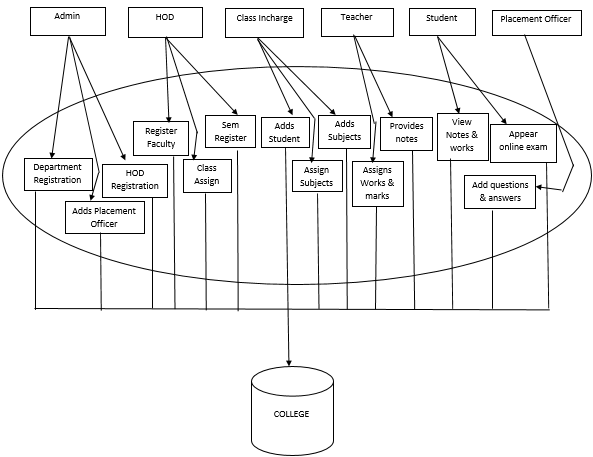
\includegraphics[width=0.5\linewidth]{Architectural}
	%\caption{}
	\label{}
\end{figure}
\newpage
\subsection{USECASE DIAGRAM}
\paragraph{}A use case diagram is a dynamic or behavior diagram in UML. Use case diagrams model the functionality of a system using actors and use cases. Use cases are a set of actions, services, and functions that the system needs to perform.A UML use case diagram is the primary form of system/software requirements for a new software program underdeveloped. Use cases specify the expected behavior (what), and not the exact method of making it happen (how). Use cases once specified can be denoted both textual and visual representation.
\begin{figure}[!htb]
\begin{center}
	\includegraphics[width=0.5\linewidth]{use1.png}
	\caption{Ideal Burn Down chart}
\end{center}
\end{figure}

\begin{figure}[!htb]
\begin{center}
	\includegraphics{use2.png}
	\caption{Ideal Burn Down chart}
\end{center}
\end{figure}
\newpage
\subsection{ACTIVITY DIAGRAM}
\paragraph{}Activity diagram is defined as a UML diagram that focuses on the execution and flow of the behavior of a system instead of implementation. It is also called object-oriented flowchart. Activity diagrams consist of activities that are made up of actions which apply to behavioral modeling technology.

\begin{figure}[!htb]
\begin{center}
	\includegraphics[width=0.5\linewidth]{home.png}
	\caption{Ideal Burn Down chart}
\end{center}
\end{figure}



\newpage
\section{AGILE TECHNOLOGY OVERVIEW  }
\subsection{ INTRODUCTION TO SCRUM}
\paragraph{}"SCRUM is a subset of agile.it is a light weight process framework for agile
development, and the ,most widely used one.A "process framework" is a particular set of practices that must be followed in order for a process to be consistant with the framework."
\subsection{ PRINCIPLES OR METHODOLOGY USED }
\paragraph{}The SCRUM methodology is defined by team rules,events(ceremonies),artifacts and roles.
\subsubsection{ The Scrum Team}

\paragraph{}A scrum team is a collection of individuals working together to deliver the requested and commited product increments.To work effectively it is important for a scrum team that everyone within the team follow a commen goal.The scrum team are typically composed of 7 +/- 2 members and have no team leaders to delegate task or decide how a problem is solved.
There are 3 roles in a scrum team:
\begin{itemize} \item The Product Owner

\paragraph{}The product owner is a project's key stakeholder-Usually an internal or external customer.or a scope person for the customer.There is only one product owner who conveys the overall mission and vision of the product which the team is building.The product owner is ultimately accountable for managing the product backlog and accepting completed increments of work.
\item The Scrum Master

\paragraph{}The scrum master is the servant leader to the product owner,development team and organization.With no hierarchichal authority over the team but rather more of a fceilitator,The scrum master ensures that the team adhers to scrum theory,practices and rules.The scrum master protect the
team by doing anything possible to help the team perform of the highest level.This may include removing impediments,fecilitating meetings and helping the product owner groom the backlog

\item The Development Team

\paragraph{}The development team is a self organizing,cross functional group armed with all of the skills to deliver shippable increments at the completion of each sprint.
\end{itemize}
\subsection{ SCRUM EVENTS}

\paragraph{}Scrum events are time boxed events that means in a project,every scrum events has a predefined maximum duration.These events enable transperancy on the project progress to all who are involved in the projects.The vital events of scrum are the Sprint.
\begin{itemize} 
\item The Sprint
\paragraph{}A sprint is a time boxed period during which specific work is completed and made ready for review.Sprint are usually 2 4 weeks long but can be as short as 1 week .
\item Sprint Planning
\paragraph{}Sprint Planning team meetings are time boxed events that determine which product backlog items will be delliverd and have the work will be achieved.
\item The daily Standup
\paragraph{}The daily stand up is a short communication meeting in which each
team member quickly and transperantly covers progress since the last stand-up ,planed work before the next meeting and any impediments that may be blocking his or her progress.
\item The Sprint Review
\paragraph{}The sprint review is the "show and tell" oe demonstration events for the team to present the work completed during the sprint.The product owner checks the work against predefined acceptance criteria or either accept or reject the work.The stakeholder or client give feedback to ensure that the deliverd incremental must the business model.
\item Retrospective
\paragraph{}The retrospective or retro is the final team meeting in the sprint to determine what went well,what didn't go well and how the team can improve the next sprint. Attended by the team and the scrum master,the retrospective is an important oppurtunity for the team to focus on its overall performance and identify startegies for continous improvement on its process.
\end{itemize}
\subsection{ SCRUM ARTIFACTS}
Scrum artifacts are designed to increase transperancy of information related to the delivary of the project, and provide oppertunities for inspection and adaptation.They are management products useful for the creation of the specialist product of the project.\\
There are 3 artificats in scrum\\
\textbf{1.} Product Backlog\\
An extended list of everything that might be needed in the final product.\\
\textbf{2.} Sprint Backlog\\
Selected items for the product backlog to be deliverd through a sprint,along with the task for delivering the item and realizing the sprint goal.\\
\textbf{3.} The Sprint Review Increment\\
set of all the product backlog items so far in the project\\.
\subsection{SCRUM RULES}
The rules of Agile Scrum Should be completely up to the team and governed for what works best for their processess.The best agile will tell teams to start with basic scrum events listed above and then inspect and adopt based on your teams unique needs so there is continous improvement in the way teams work together.
\section{SPRINT }

\subsection{PRODUCT BACKLOG}

\paragraph{}
In the simplest definition the Scrum Product Backlog is simply a list of all things that needs to be done within the project. It replaces the traditional requirements specification artefacts. These items can have a technical nature or can be user-centric e.g. in the form of user stories.Product Backlog refinement is the act of adding detail, estimates, and order to items in the Product Backlog. This is an ongoing process in which the Product Owner and the De- development Team collaborate on the details of Product Backlog items.A Scrum product backlog contains descriptions of the functionality desired in an end product. Agile backlog prioritization is the next step.
\paragraph{}
The Product Backlog is the tool used by the product owner to keep track of all of the features that stakeholders would like to see implemented in the product whereas the Sprint Backlog is a subset of the Product Backlog representing the current active Sprint iteration. ... However, the product owner prioritizes it.


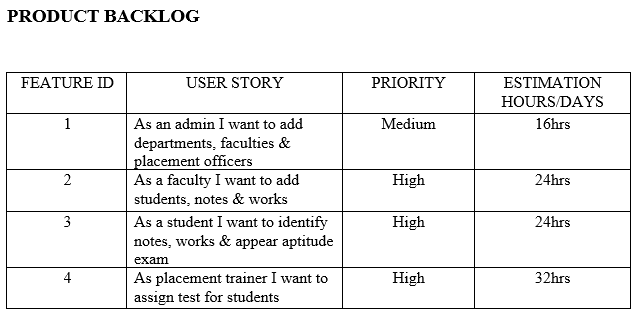
\includegraphics[scale=1]{product} 
\subsection{SPRINT PLANNER}

\paragraph{}
Sprint Planning is time-boxed to a maximum of eight hours for a one-month Sprint. For shorter Sprints, the event is usually shorter. The Scrum Master ensures that the event takes place and that attendants understand its purpose. The Scrum Master teaches the Scrum Team to keep it within the time-box.The Sprint Goal is an objective set for the Sprint that can be met through the implementation of Product Backlog. It provides guidance to the Development Team on why it is building the Increment. It is created during the Sprint Planning meeting. The Sprint Goal gives the Development Team some exibility regarding the functionality implemented within the Sprint. As the Development Team works, it does so with the Sprint Goal always in mind.


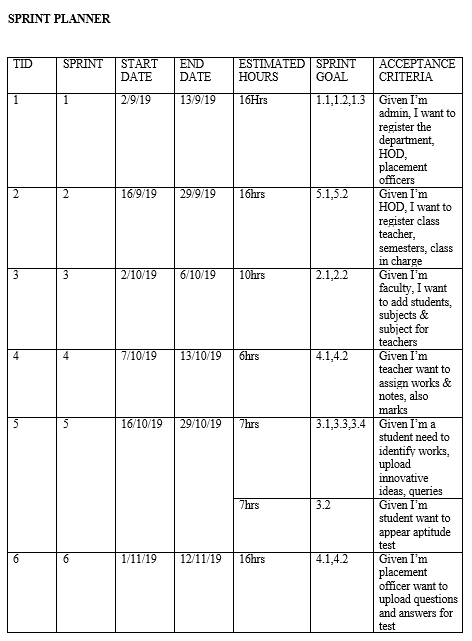
\includegraphics[scale=1]{sprint} 

\subsection{IDEAL BURN DOWN CHART}

\paragraph{}
A burn down chart is a graphical representation of work left to do versus time. The outstanding work (or backlog) is often on the vertical axis, with time along the horizontal. That is, it is a run chart of outstanding work. It is useful for predicting when all of the work will be completed. It is often used in agile software development methodologies such as Scrum. However, burn down charts can be applied to any project containing measurable progress over time.One issue that may be noticed in burn down charts is that whether or not the Actual Work line is above or below the Ideal Work line depends on how accurate the original time estimates are. This means that if a team constantly overestimates time requirements, the progress will always appear ahead of schedule. If they constantly underestimate time requirements, they will always appear behind schedule.
\begin{figure}[ht]
	\centering
	\includegraphics[width=1.0\linewidth]{ideal}
	%\caption{}
	\label{}
\end{figure}


 
\subsection{ GIT HUB REGISTRATION}
GitHub is an online-browser based distributed version control system for software developers using the Git revision control system. The service provides free public repositories, issue tracking, graphs, code review, downloads, wikis, collaborator management, and more.GitHub offers free accounts for users and organizations working on public and open source projects, as well as paid accounts that offer unlimited private repositories and optional user management and security features.Git hub account creation includes the following steps:
 \begin{itemize}
 
 \item Go to the GitHub sign up page,then  Enter a username, valid email address, and password. Use at least one lowercase letter, one numeral, and seven characters.
 \item Review carefully the GitHub Terms of Service and Privacy Policy before continuing and Choose a plan. Hereby anyone can finish the account creation procedure.
 \item  You can store a variety of projects in GitHub repositories, including open source projects. 
 \item In the upper-right corner of any page, click , and then click New repository.
 \item Type a short, memorable name for your repository followed by Optionally, add a description of your repository,public or private repository.
 \item Select Initialize this repository with a README.finally Click Create repository.
 \item After creation, need to collaborate members by the admin. 
 \item In the left sidebar, click Collaborators and teams.
 \item Under "Collaborators",type the name of the person you'd like to give access to the repository, then click Add collaborator.
 \item Next to the new collaborators name, choose the appropriate permission level: Write, Read, or Admin. 
 \item The user will receive an email inviting them to the repository. Once they accept your invitation, they will have collaborator access to your repository.
 \end{itemize} 

\section{SYSTEM DESIGN}


\subsection{HARDWARE AND SOFTWARE SPECIFICATION}
\begin{itemize}
\item HARDWARE REQUIREMENTS
\paragraph{}In order to implement a new system thee choice of a processor with maximum
possible speed is maid. There should be sufficient memory to store data and software tools
for efficient processing.
\begin{itemize}
\item System : DESKTOP-5VKB9RT
\item Processor : Pentium III or above
\item Memory : 1GB or above
\item Hard Disk : 80 GB or above
\end{itemize}

\item  SOFTWARE REQUIREMENTS
\begin{itemize}
\item Operating System : Windows 7 or above, macOS, and Linux.
%\item IDE : 
%\item Complier : 
\item Framework : Django
\item Scripting Language :Python* versions: 2.7.X, 3.6.X
\item Database : SQLite
\end{itemize}
\end{itemize}
%\subsection{NETWORK CONNECTIVITY OR SPECIAL REQUIREMENTS}
\subsection{TECHNOLOGY}
\begin{itemize}
\item FRONT END
\item BACK END
\item GIT AND SOFTWARE TOOLS 
\end{itemize}
\subsection{MODULE DESCRIPTION}
\begin{enumerate}
\item \textbf{Admin}
\paragraph{}Admin panel in the college management system enables easy supervision of all the administrative activities of the college by the authorized users.All the functions of the management system can be operated from the admin panel and access can be provided to different users.The authorized users can manage a wide range of activities of the system from anywhere and anytime by logging in their accounts. The privileges for each user can be assigned through this admin panel.Admin will add the departments in the college, HODs for each department and also register the placement officers.The admin can view the feedback provided by the students. 
\item \textbf{HOD}\paragraph{}HOD can handle the department. When they login to their account they can perform the functionalities provided for them. They first of all need to register the semsters in the department then add the faculties in the department. HODs can assign class incharge for each semesters.
\item \textbf{Faculty}\paragraph{}When the faculties login to the system they can perform their functionalities provided. They add the subjects in a course. They assign other faculties for each subject. The faculties will assign works for the class. They provide mark for the students work .
\item \textbf{Students}\paragraph{} When students  login to the system they can view notes and notification of works provided by the teachers .work may be online or offilne.There is an area for the completion of the work.They can provide innovative ideas.
\item \textbf{Placement Cell Officer}Placement cell officer is responsible for providing the aptitude test for the students .And he/she can add other faculties.Students can  appear on  the test and they can make self assessments.
\end{enumerate}
\subsection{INPUT DESIGN}
\paragraph{}
Input design converts user-oriented inputs to computer- based format, which requires careful attention. The collection of input data is the most expensive part of the system in terms of the equipment used and the number of people involved. In input design, data is accepted for computer processing and input to the system is done through mapping via some map support or links.The input screens need to be designed very carefully and logically. A set of menus is provided which help for better application navigation. While entering data in the input forms, proper validation checks are done and messages will be generated by the system if incorrect data has been entered.
\paragraph{}
In this project,each module have its own input screens and value insert from option box.For example,result page will display results of students.
\subsection{DATABASE DESIGN}
\paragraph{}
Data design is the first and most important design activity. Here the main issue is to select the appropriate data structure. That is the Data design focuses on the definition of data structures.
\paragraph{}
Database design is required to manage the large bodies of information. The management of data involves both the definition of structure of the storage information and provisions of mechanism for the manipulation of information. In addition the database system must provide for the safety of information handled, despite the system crashes due to attempts art unauthorized access. For developing an efficient database, we will have to fulfill certain condition such as:\\
\fontsize{12pt}{12pt}\selectfont
\textbf{- }Control redundancy.\\
\textbf{- }Ease of use.\\
\textbf {- }Data independence.\\
\textbf{- }Accuracy and integrity.\\
\textbf{- }Avoiding in ordinate delays.\\
\textbf{- }Recovery from failure.\\
\textbf{- }Privacy and security.\\
\subsection{TABLE DESIGN}
\paragraph{}This is one of the major tasks in designing the database. It is important to realize that
the design of the system is totally inter-related and so table design of the system is totally
inter-related and so table design cannot really be considered in isolation from inputs, outputs,
procedures, codes and security requirements.The system can
extract information whenever necessary using the Structured Query Language (SQL).
\\
\textbf{NORMALIZATION}
\paragraph{}The term normalization of data refers to the way data items are grouped together into
record structures. Normalizations are used to overcome the drawbacks like repetition of
data, loss of information and consistency. In the real life data exists as a collection of data.
Data structuring is refined through the process called normalization. These groups are
normally not in a normalized form. Without normalization, if implemented, many
drawbacks can arise. Various normal forms are available. The basic objective of
normalization is to reduce the data redundancy. That means that, information is stored only
once. Mainly important types of normal forms are:\\
\textbf{FIRST NORMAL FORM}
\paragraph{} A relation is said to be in first normal form if the values in the relation are atomic for
every attribute in the relation. By this we mean simply that no attribute value can be a set of
values or, as it is sometimes expressed, a repeating group.\\
\textbf{SECOND NORMAL FORM}
\paragraph{}A relation is said to be in second Normal form is it is in first normal form and it
should satisfy any one of the following rules.
\begin{itemize}
\item Primary key is a not a composite primary key
\item No non key attributes are present
\item Every non key attribute is fully functionally dependent on full set of primary
\end{itemize}
\textbf{THIRD NORMAL FORM}\\
\paragraph{}A relation is said to be in third normal form if their exits no transitive dependencies.
Transitive Dependency: If two non-key attributes depend on each other as well as on the
primary key then they are said to be Transitive dependent.
\paragraph{}The above normalization principles were applied to second normal form to
decompose the data in multiple tables thereby making the data to be maintained in a
consistent state.
\paragraph{}The Database contains the following tables.\\
\textbf{TABLES}

{\fontsize{14pt}{14pt}\selectfont\textbf{1.Login Table}
\\
\\
\begin{tabular}{|c|c|c|c|}
\hline 

FIELD NAME&DATA TYPE\\

\hline 

Username&Varchar\\ 
\hline 
Password&Varchar \\ 
\hline 
Role&varchar\\
\hline

\end{tabular} }\\
\\
\\
\\{\fontsize{14pt}{14pt}\selectfont\textbf{2.Department Table}
\\
\\
\begin{tabular}{|c|c|c|c|}
\hline 
FIELD NAME&DATA TYPE\\
Loginid&integer\\
\hline 
Deptid&integer\\
\hline
Deptname&varchar\\
\hline
\end{tabular} 
\\{\fontsize{14pt}{14pt}\selectfont\textbf{3.Faculty Table}
\\
\\
\begin{tabular}{|c|c|c|c|}
\hline 
FIELD NAME&DATA TYPE\\
Teachid&Integer\\
\hline 
Name&Varchar\\
\hline
Email&Varchar\\
\hline
Username&Varchar\\
\hline
Password&Varchar\\
\hline
Address&Varchar\\
\hline
Phone&Varchar\\
\hline
Address&Varchar\\
\hline
Dept&Varchar\\
\hline
Gender&Varchar\\
\hline
Loginid&Integer\\
\hline
Deptid&Integer\\
\hline

\end{tabular} 
\\{\fontsize{14pt}{14pt}\selectfont\textbf{4.Sem Table}
\\
\\
\begin{tabular}{|c|c|c|c|}
\hline 
FIELD NAME&DATA TYPE\\
Semid&Integer\\
\hline 
Sem&Varchar\\
\hline
\end{tabular}
\\{\fontsize{14pt}{14pt}\selectfont\textbf{5.HOD Table}
\\
\\
\begin{tabular}{|c|c|c|c|}
\hline 
FIELD NAME&DATA TYPE\\
Hodid&Integer\\
\hline 
Name&Varchar\\
\hline
Email&Varchar\\
\hline
Username&Varchar\\
\hline
Password&Varchar\\
\hline
Address&Varchar\\
\hline
Phone&Varchar\\
\hline
Address&Varchar\\
\hline
Dept&Varchar\\
\hline
Gender&Varchar\\
\hline
Loginid&Integer\\
\hline
Deptid&Integer\\
\hline

\end{tabular}  

\subsection{INPUT DESIGN WITH VALIDATIONS}
\subsection{REPORT}
\newpage
\section{CODING}
\subsection{CODING STANDARDS USED IN HE PROJECT}
\fontsize{12pt}{12pt}\selectfont
\lstinputlisting{./py.txt}
\newpage
\section{TESTING}
\paragraph{}Testing is a process of executing a program with the interest of finding an error. A good
test is one that has a high probability of finding the yet undiscovered errors. The primary
objective for the test case design is to drive a set of tests that has the highest likelihood for
systematically uncovering different classes of errors in the software. Testing begins at the
level and works outward towards the interaction of the entire software. A series of testing are
performed for this project before the system is ready for acceptance.
\subsection{UNIT TESTING}
\paragraph{}In this testing we test each module individual and integrated the overall system. Unit
testing focuses verification efforts on the smaller unit of software design in the module. This
is also known as ‘module’ testing. The modules of the system are tested separately. The
testing is carried out during programming stage itself. In this testing step each module is
found to working satisfactory as regard to the expected output from the module. There are
some validation checks for verifying the data input given by the user which both the formal
and validity of the entered. It is very easy to find error debug the system. In our application
we are could invalid forms and check there is any proble.m
\subsection{OTHER TESTING STRATEGIES USED}
\begin{itemize}
\item Integration Testing
\paragraph{} Integration testing is the systematic testing for constructing the uncover errors within
the interface. This testing was done with sample data. The developed system has run
successful for this sample data. The need for integrated test is to find the overall system
performance. Integration testing is performing after the successful completion of unit testing.
\item Validation Testing
\paragraph{}Software is completely assembled as a package, interface errors have been uncovered
and corrected and final series of software tests, validation tests begins. Validation testing can
be defined many, but a simple definition is that validation succeeds when the software
functions in a manner that can be reasonably accepted by the customer.
\item Output Testing
\paragraph{}After performing the validation testing, the next step is output testing of the proposed system
since no system could be useful if it doesn’t produce the required data in the specific format.
The output displayed or generated by the system under consideration is tested by, checking
with the format displayed. The output format on the screen is found to be correct as the
format was designed in the system phase according to the design. Hence the output testing
doesn’t result in any correction in the system, except the format of the output displayed.
\end{itemize}
\newpage


\section{IMPLEMENTATIONS}
\paragraph{}
	After the system has been tested, the implementation type or the change over technique from the existing system to the new system is a step-by-step process. In the system at first only a module of the system is implemented and checked for suitability and efficiency. When the end user related to the particular module is satisfied with the performance, the next step of implementation is preceded.
	\paragraph{}
Implementation to some extent is also parallel. For instance, modules which are not linked, with other modules are implemented parallel and the training is the step-by -step process.Backups are necessary since any time unexpected events may happen. And so during the program execution, the records are stored in the workspace. This helps to recover the original status of the records from any accidental updating or intentional deletion of records.

\subsection{IMPLEMENTATION METHOD USED}
The implementation stage involves following tasks: \\
\linebreak
\textbf{- }Careful planning \\
\textbf{- }Investigation of system and constraints \\
\textbf{- }Design of method to achieve the changeover phase \\
\textbf{- }Evaluation of the changeover method \\
%\begin{itemize}

\section{BUSINESS PERSPECTIVE}


\section{FUTURE SCOPE}
\paragraph{}It's easy to made changes and additions to website, by using MVC the Model part does not depend on the views part. Therefore, any changes in the Model will not affect the entire architecture. so anyone can easily understand the project.Online examination module would be introduced to conduct online examination.
Further, the faculty can upload the notes of their lectures on this site and students who had missed those classes can access the notes.   
\section{CONCLUSION}
The project report entitled "COLLEGE ACADEMIC MANAGEMENT" has come to its final stage. The system has been developed with much care that it is free of errors and at the same time it is efficient and less time consuming. The important thing is that the system is robust. We have tried our level best to make the site as dynamic as possible. Also provision is provided for future developments in the system. The entire system is secured. This online system will be approved and implemented soon. 

\newpage
\section{APPENDIX}
\subsection{GIT HISTORY}
\subsection{SCREENSHOTS}
\begin{figure}[!htb]
\begin{center}
	\includegraphics[width=450pt,height=400pt]{home.png}
	\caption{Ideal Burn Down chart}
\end{center}
\end{figure}

\newpage

\subsection{SAMPLE TEMPLATE FOR SPRINT BACKLOG, DAILY SCRUM}
\begin{figure}
	\centering
	\includegraphics[width=1.0\linewidth]{actual}
	%\caption{HOD Page}
	\label{}
\end{figure}
\subsection{SAMPLE CODE}
\fontsize{12pt}{12pt}\selectfont
\lstinputlisting{./views.py}



\newpage
\section{BIBLIOGRAPHY}
\fontsize{12pt}{12pt}\selectfont
\lstinputlisting{./reference.txt}
\end{document}